\documentclass[14pt]{article}
\usepackage[utf8]{inputenc}
\usepackage{graphicx}
\usepackage{siunitx}
\usepackage[table]{xcolor}
\usepackage{amsmath}
\usepackage{geometry}
\geometry{a4paper,
 total={170mm,257mm},
 left=30mm,
 right=30mm,
 bottom=40mm,
 top=44mm}

\sisetup{
    group-separator={,},
    group-minimum-digits=3,
    round-mode=places,
    round-precision=2,
    table-format=3.2
}

\title{\textbf{Gear Ratio Calculation Report}}

\author{\textbf{Doc-No.: {{ doc_no | default('—') }}}\\
Made By: {{ made_by | default('—') }}\\
Checked By: {{ checked_by | default('—') }}\\
Approved By: {{ approved_by | default('—') }}}
\date{{ doc_date | default("\\today") }}

% Background logos (added with safety guard)
\usepackage{eso-pic}
\IfFileExists{logo.JPG}{
  \AddToShipoutPictureBG{
    \AtPageUpperLeft{\raisebox{-\height}{
\includegraphics[width=\paperwidth]{logo.JPG}}}
    \IfFileExists{logo-1.JPG}{\AtPageLowerLeft{\makebox[\paperwidth]{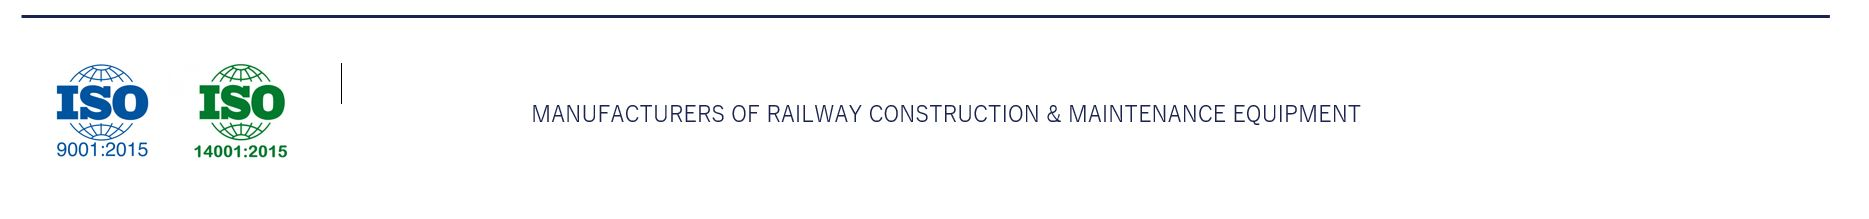
\includegraphics[height=2.3cm]{logo-1.JPG}}}}{}
  }
}{}

\begin{document}
\maketitle

\section*{Introduction}
This report computes the required gear ratio to meet a target vehicle speed given motor RPM limits and wheel size.

\section{Theory and Formulas}
\begin{itemize}
  \item Wheel circumference: $C = \dfrac{wheel\_dia \times \pi}{1000}$ (m)
  \item Speed (m/s): $V = V_{km/h} \times 1000 / 3600$
  \item Wheel RPM: $RPM_{wheel} = \dfrac{V}{C} \times 60$
  \item Required gear ratio: $gear = \dfrac{max\_motor\_rpm}{RPM_{wheel}}$
\end{itemize}

\section{Inputs}
\begin{itemize}
  \item Target Speed = {{ speed | default('N/A') }} km/h
  \item Wheel Diameter = {{ wheel_diameter | default('N/A') }} mm
  \item Max Motor RPM = {{ max_motor_rpm | default('N/A') }} RPM
\end{itemize}

\section{Calculation}
\subsection*{Derivation (symbolic)}
Let $C$ be wheel circumference, $V$ the vehicle speed (m/s), and $RPM_{wheel}$ the wheel RPM. Then:
\[ C = \frac{wheel\_dia \times \pi}{1000}, \quad V = V_{km/h} \times \frac{1000}{3600} \]
\[ RPM_{wheel} = \frac{V}{C} \times 60, \quad Required\ Gear\ Ratio = \frac{max\_motor\_rpm}{RPM_{wheel}} \]

\subsection*{Worked numeric substitution}
Wheel circumference:
\[ C = \frac{ {{ wheel_diameter | default(0) }} \times \pi }{1000} = {{ wheel_circumference | default(0) | round(3) }} \, m \]
Convert speed to m/s:
\[ V = {{ speed | default(0) }} \times \frac{1000}{3600} = {{ speed_mps | default(0) | round(2) }} \, m/s \]
Wheel RPM required:
\[ RPM_{wheel} = \frac{ V }{ C } \times 60 = {{ wheel_rpm | default(0) | round(2) }} \, RPM \]
Required gear ratio:
\[ Required\ Gear\ Ratio = \frac{ {{ max_motor_rpm | default(0) }} }{ {{ wheel_rpm | default(0) | round(2) }} } = {{ required_gear_ratio | default(0) | round(3) }} \]

\subsection*{Sensitivity analysis (±10%)}
\begin{itemize}
  \item If wheel diameter increases by +10\% → wheel circumference increases by +10\%, wheel RPM decreases by ≈10\% → required gear ratio increases by ≈10\%.
  \item If max motor RPM changes by ±10\% the required gear ratio scales inversely (directly proportional to max motor RPM).
\end{itemize}

\section{Summary}
\begin{itemize}
  \item Required gear ratio (motor_rpm / wheel_rpm): \textbf{ {{ required_gear_ratio | default(0) | round(3) }} }
  \item Wheel RPM at target speed: \textbf{ {{ wheel_rpm | default(0) | round(2) }} RPM }
\end{itemize}

\subsection*{Appendix: trace}
\begin{itemize}
  \item Wheel circumference = {{ wheel_circumference | default(0) | round(3) }} m
  \item Vehicle speed (m/s) = {{ speed_mps | default(0) | round(2) }} m/s
  \item Wheel RPM = {{ wheel_rpm | default(0) | round(2) }} RPM
  \item Max motor RPM = {{ max_motor_rpm | default('N/A') }} RPM
  \item Required gear ratio = {{ required_gear_ratio | default(0) | round(3) }}
\end{itemize}

\end{document}
